% METODOLOGIA------------------------------------------------------------------

\chapter{PROPOSTA}
\label{chap:proposta}
Neste capítulo será elaborada a proposta de desenvolvimento do projeto, tecnologias e metodologias a serem utilizadas.

\section{PÚBLICO-ALVO}
Identificou-se como público-alvo para o projeto desenvolvido o conjunto de diretores e demais profissionais responsáveis pela elaboração de grades horárias em escolas de ensino fundamental e médio. Quanto à dimensão das instituições de ensino, o trabalho visa contemplar aquelas de pequeno e médio porte.

\section{TECNOLOGIAS E FERRAMENTAS}
Como mencionado anteriormente, o presente trabalho tem como objetivo o desenvolvimento de uma aplicação que automatize e simplifique o processo de criação de grades horárias escolares. Para concluir este objetivo, optou-se por desenvolver uma aplicação que execute no servidor, com uma interface \textit{web} para interação com o usuário. 

Vale ressaltar que inicialmente as premissas do problema e informações encontradas na literatura foram utilizadas para nortear o levantamento de requisitos e o desenvolvimento inicial da aplicação. Estes requisitos serão complementados e ajustados de acordo com os dados coletados de potenciais usuários futuros, conforme o critério metodológico exposto na seção \ref{chap:introducao}.

As tecnologias e ferramentas a serem utilizadas são:

\begin{itemize}
	\item \textbf{VSCode}: Editor de código-fonte desenvolvido pela Microsoft, escolhido por sua versatilidade e aplicabilidade para desenvolver todos os componente do sistema
	\item \textbf{DBeaver}: Ferramenta de código aberto de administração de bancos de dados, utilizada para validação da modelagem e interações manuais com a base de dados
	\item \textbf{PostgreSQL}: Sistema gerenciador de banco de dados relacional, escolhido por sua robustez, possibilitará a persistência dos dados da aplicação em tabelas
	\item \textbf{JavaScript}: Linguagem de programação ubíqua na engenharia de software, escolhida por sua versatilidade para desenvolver a interface \textit{web} e servidor
	\item \textbf{VueJS}: \textit{Framework} para desenvolvimento frontend na linguagem JavaScript, escolhido por sua versatilidade e familiaridade do graduando com este
	\item \textbf{VuetifyJS}: \textit{Framework} de componentes e estilização para o VueJS, utilizado para padronizar o design da aplicação
	\item \textbf{NodeJS}: \textit{Runtime} de JavaScript que permite a utilização dessa linguagem para escrever aplicações no lado do servidor;
	\item \textbf{ExpressJS}: \textit{Framework} para desenvolvimento backend na lignuagem JavaScript, utilizando a plataforma NodeJS
	\item \textbf{C++}: Liguagem de programação compilada, escolhida por sua alta performance para o desenvolvimento do otimizador
	\item \textbf{G++}: Compilador utilizado para converter o código fonte em C++ do otimizador para um arquivo executável 
	\item \textbf{GDB}: Debugador da linguagem C++, utilizado para localizar problemas no código fonte do otimizador
\end{itemize}

\section{ANÁLISE E DESENVOLVIMENTO}
\label{sec:analise_e_desenvolvimento}

\subsection{Interface}
A interface \textit{web} será responsável pela interação do usuário final com a aplicação. Portanto, deverá implementar funcionalidades que possibilitem a configuração das restrições e características das grades horárias a serem geradas, além de mostrar ou exportar tais grades após a geração.

Para o desenvolvimento deste componente, optou-se pelo framework \textit{Vue.js}, devido à riqueza de seu ecossistema de desenvolvimento \textit{frontend} e familiaridade do graduando com este. Complementando este framework, será utilizado também o \textit{Vuetify.js}, a fim de facilitar e padronizar o design da aplicação.

A \autoref{fig:diagrama-uc} mostra os casos de uso que a interface \textit{web} será responsável por disponibilizar:

\begin{figure}[!htb]
	\centering
	\caption{Diagrama de Casos de Uso}
	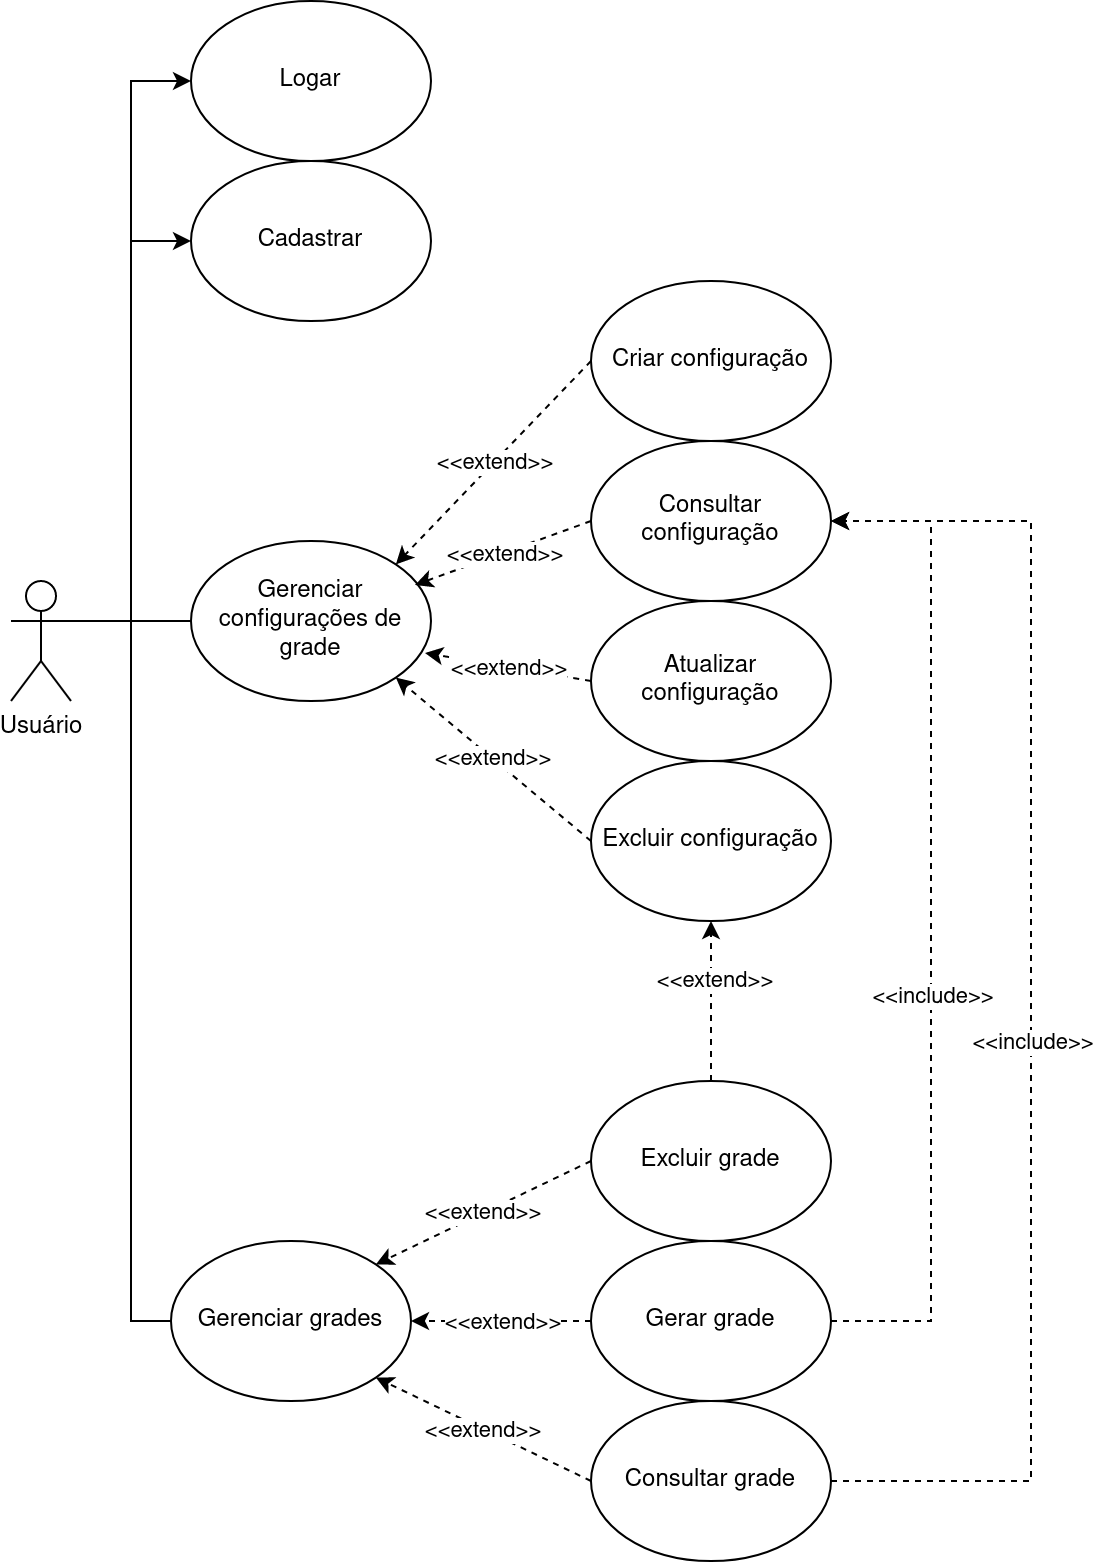
\includegraphics[width=0.65\textwidth]{./dados/figuras/diagrama_uc}
	\fonte{Autor}
	\label{fig:diagrama-uc}
\end{figure}
\newpage

Desenvolveram-se alguns protótipos iniciais das telas necessárias na aplicação.
Primeiramente, a \autoref{fig:tela-configuracoes} mostra a tela de listagem de configurações de grade. Como comentado anteriormente, alguns dos casos de uso da aplicação envolvem o gerenciamento de configurações de grades horárias, as quais são listadas nessa tela.

\begin{figure}[!htb]
	\centering
	\caption{Tela - Listagem de Configurações de Grade}
	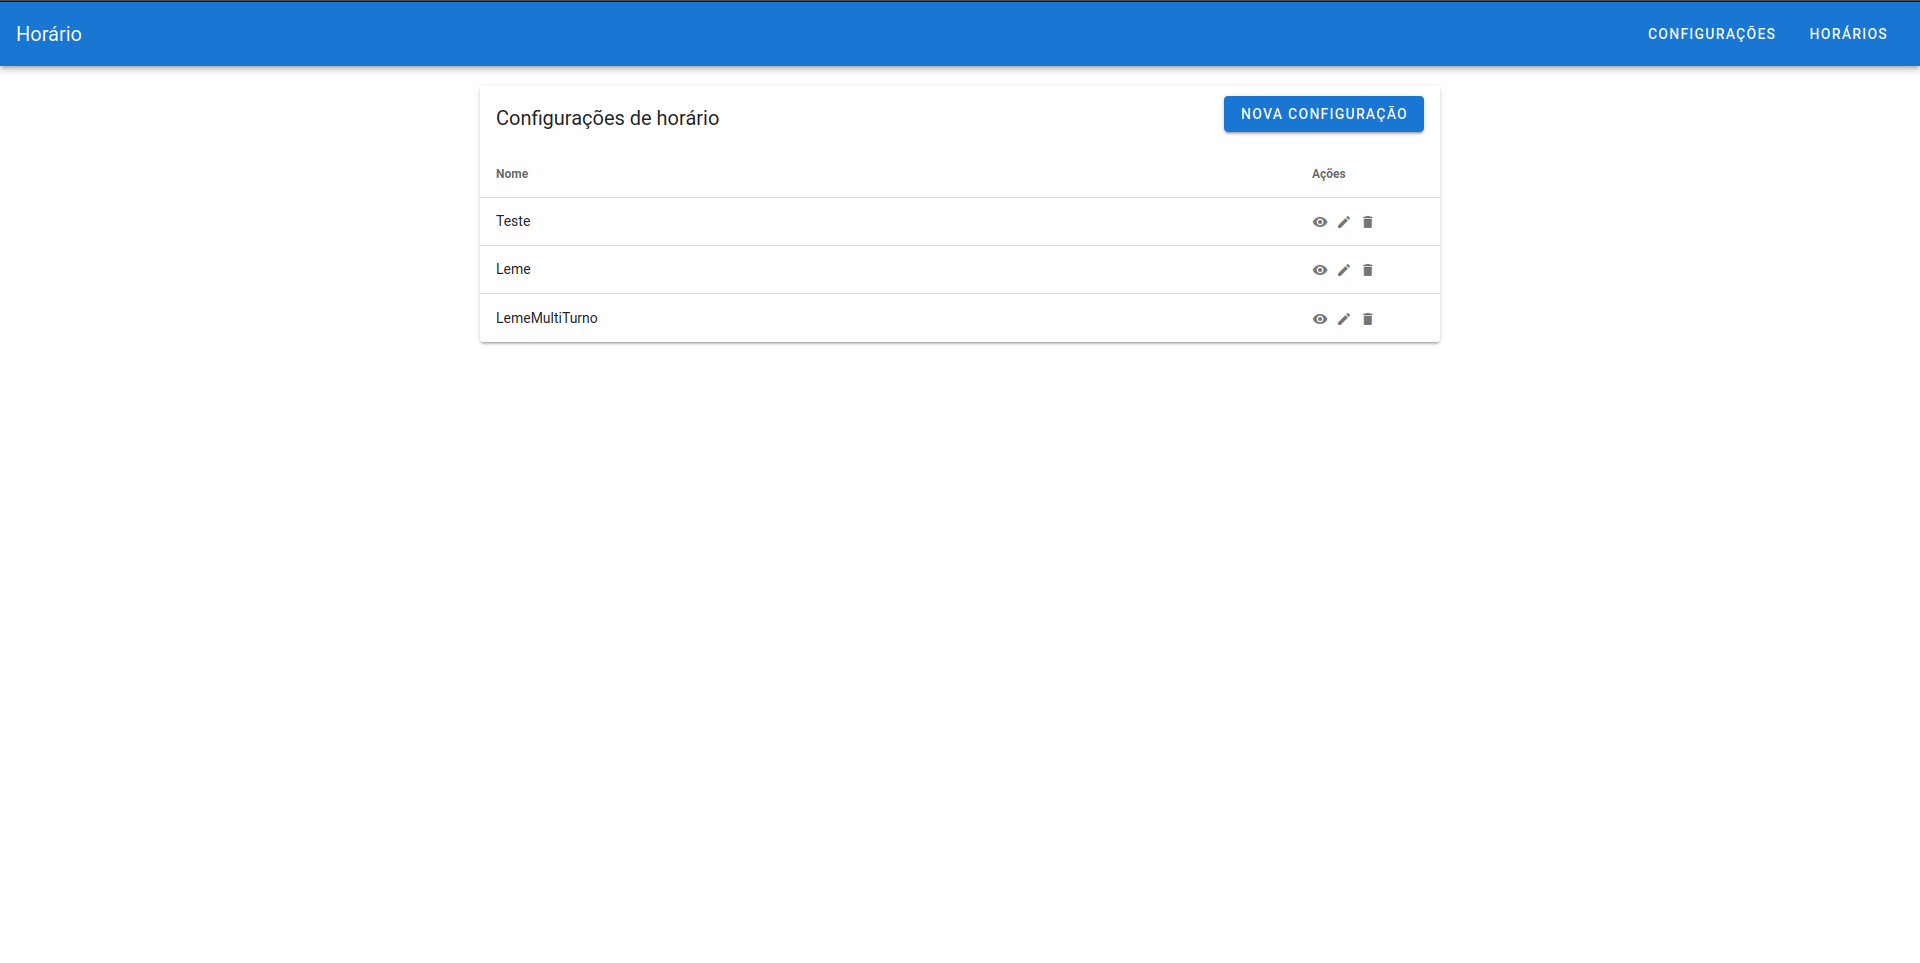
\includegraphics[width=0.8\textwidth]{./dados/figuras/tela_configuracoes}
	\fonte{Autor}
	\label{fig:tela-configuracoes}
\end{figure}

A tela mostrada na \autoref{fig:tela-estrutura1} é responsável por permitir que o usuário cadastre os professores da escola. Nessa tela é possível notar que a aplicação foi estruturada seguindo uma noção de etapas de configuração até a geração da grade horária final. No topo da tela, a etapa "Estrutura da Escola" encontra-se selecionada.

\begin{figure}[!htb]
	\centering
	\caption{Tela - Estrutura da Escola - Professores}
	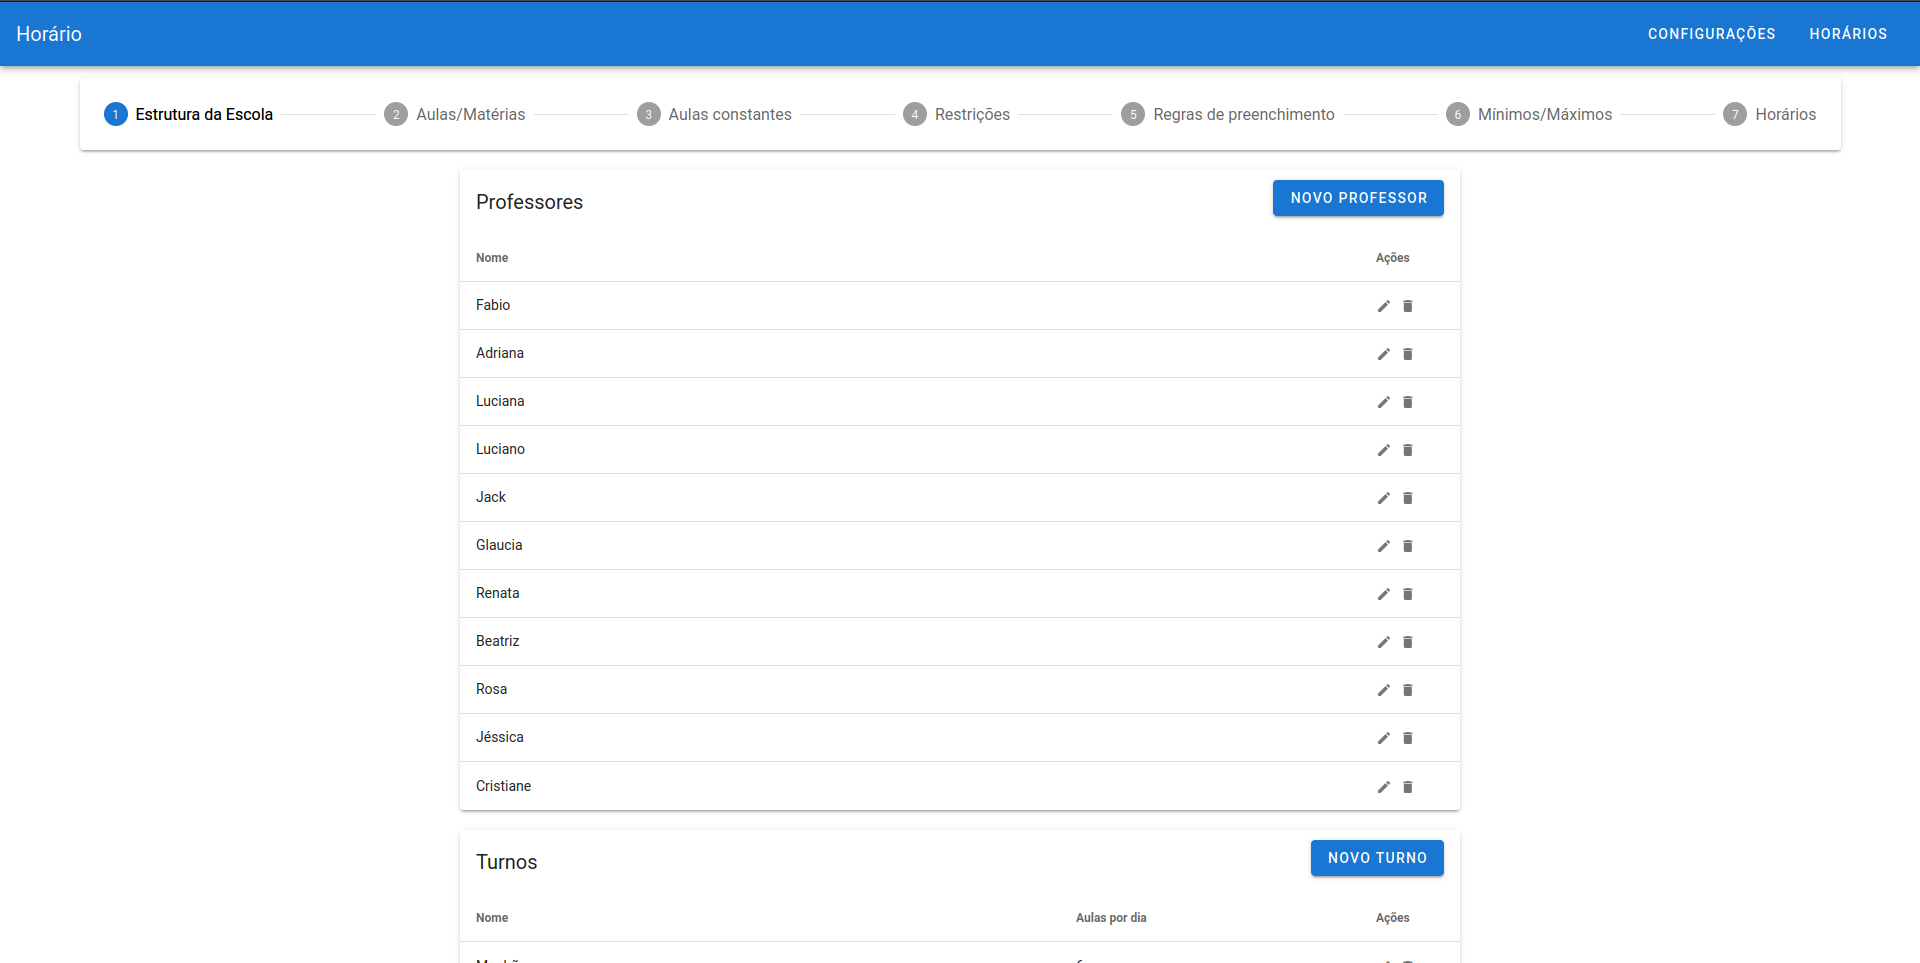
\includegraphics[width=0.8\textwidth]{./dados/figuras/tela_estrutura1}
	\fonte{Autor}
	\label{fig:tela-estrutura1}
\end{figure}
\newpage

Na \autoref{fig:tela-estrutura2}, tem-se a continuação da tela de estrutura da escola, mostrada na \autoref{fig:tela-estrutura1}. Esta parte da tela é responsável pela configuração das salas e turnos da escola.

\begin{figure}[!htb]
	\centering
	\caption{Tela - Estrutura da Escola - Salas e Turnos}
	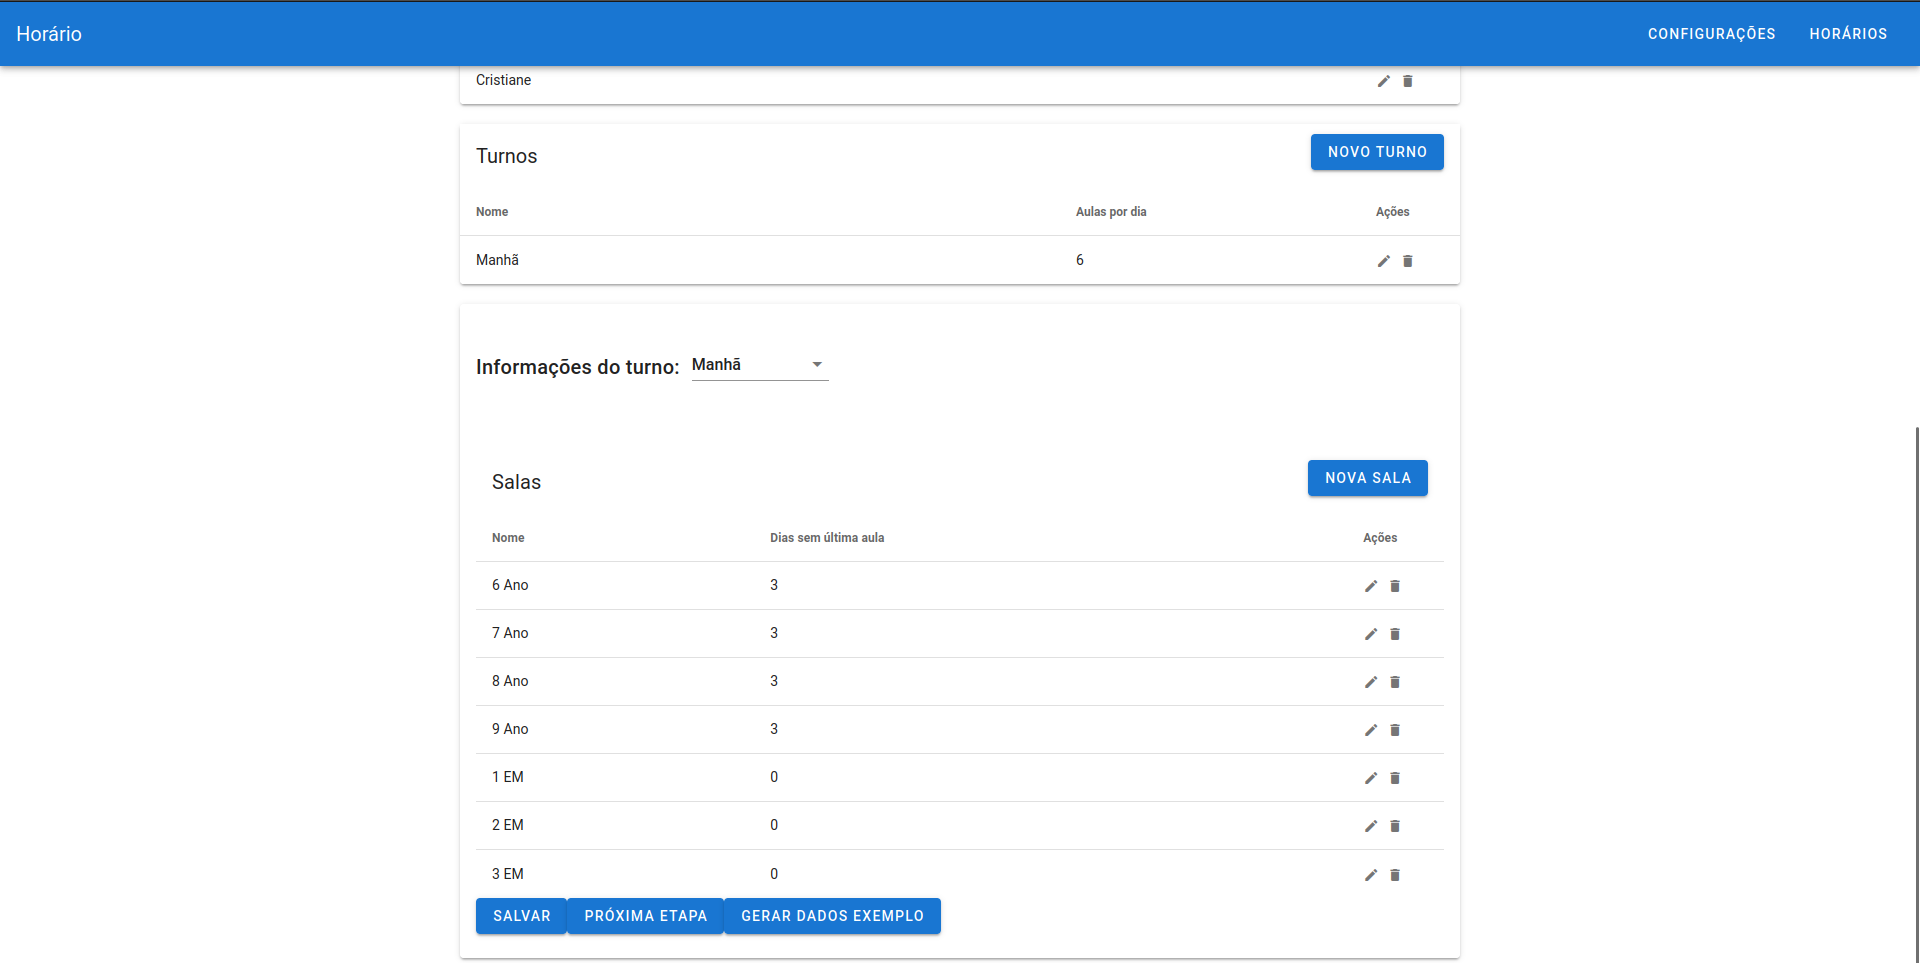
\includegraphics[width=0.8\textwidth]{./dados/figuras/tela_estrutura2}
	\fonte{Autor}
	\label{fig:tela-estrutura2}
\end{figure}

Na tela da \autoref{fig:tela-aulas}, o usuário pode realizar a configuração de número de aulas que cada professor deve ministrar em cada sala, informação fundamental para a geração das grades horárias.

\begin{figure}[!htb]
	\centering
	\caption{Tela - Aulas por professor}
	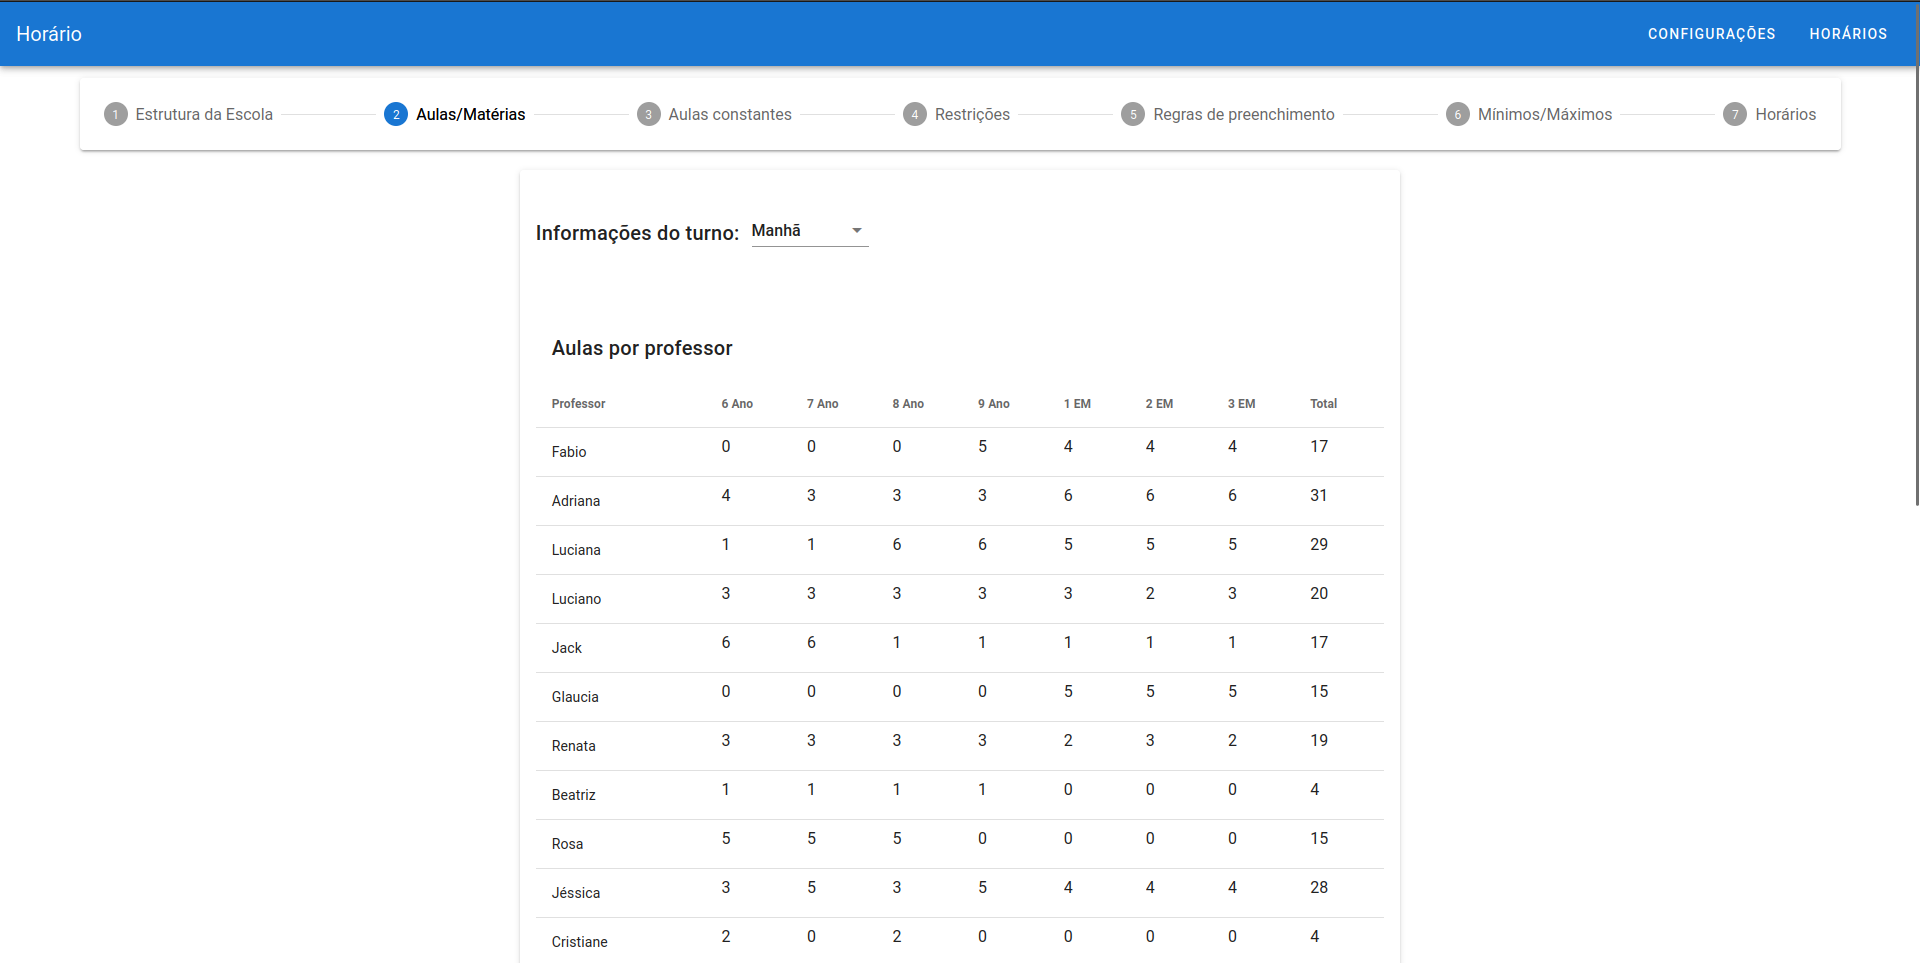
\includegraphics[width=0.8\textwidth]{./dados/figuras/tela_aulas}
	\fonte{Autor}
	\label{fig:tela-aulas}
\end{figure}
\newpage

A tela da \autoref{fig:tela-restricoes} é responsável pela configuração das restrições. Nesta, o usuário pode configurar horários na grade que devem ser evitados ou proibidos para determinado docente.

\begin{figure}[!htb]
	\centering
	\caption{Tela - Restrições}
	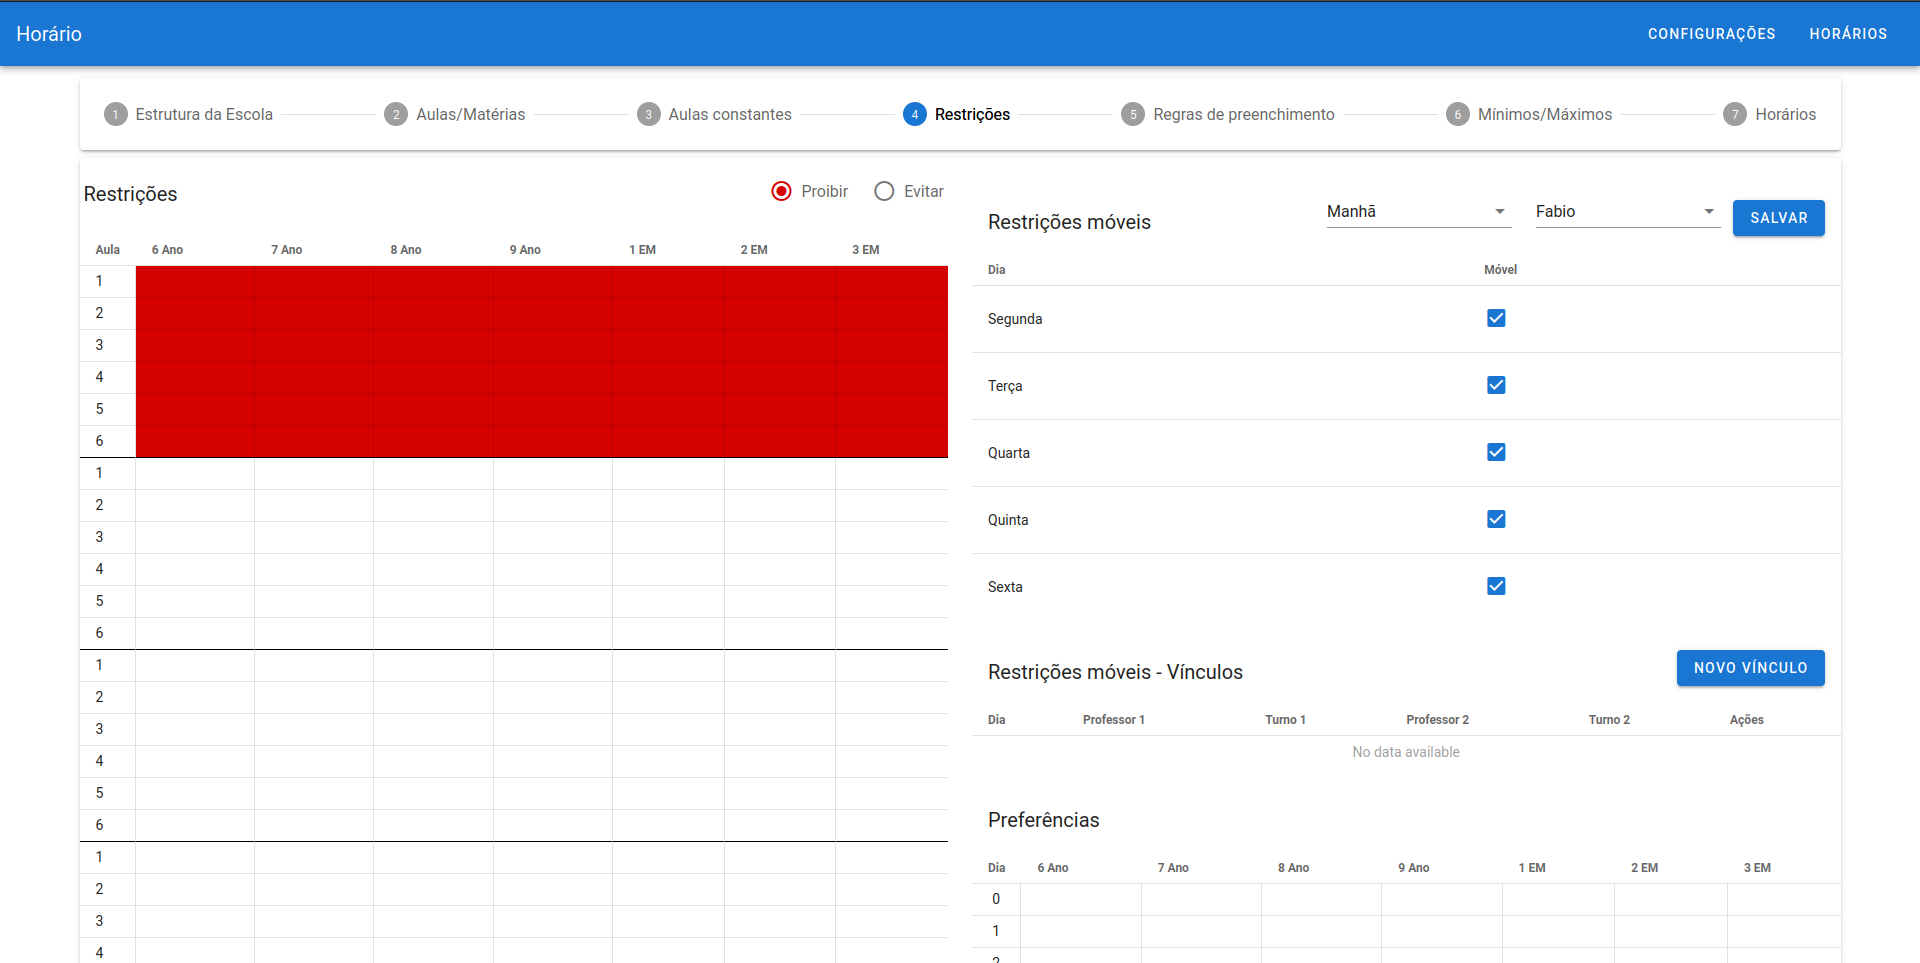
\includegraphics[width=0.8\textwidth]{./dados/figuras/tela_restricoes}
	\fonte{Autor}
	\label{fig:tela-restricoes}
\end{figure}

A última etapa no fluxo da aplicação é representada pela tela da \autoref{fig:tela-horarios}. Nesta, o usuário pode requisitar a geração da grade horária utilizando as configurações realizadas nas etapas anteriores, e acessar as grades geradas anteriormente.

\begin{figure}[!htb]
	\centering
	\caption{Tela - Horários}
	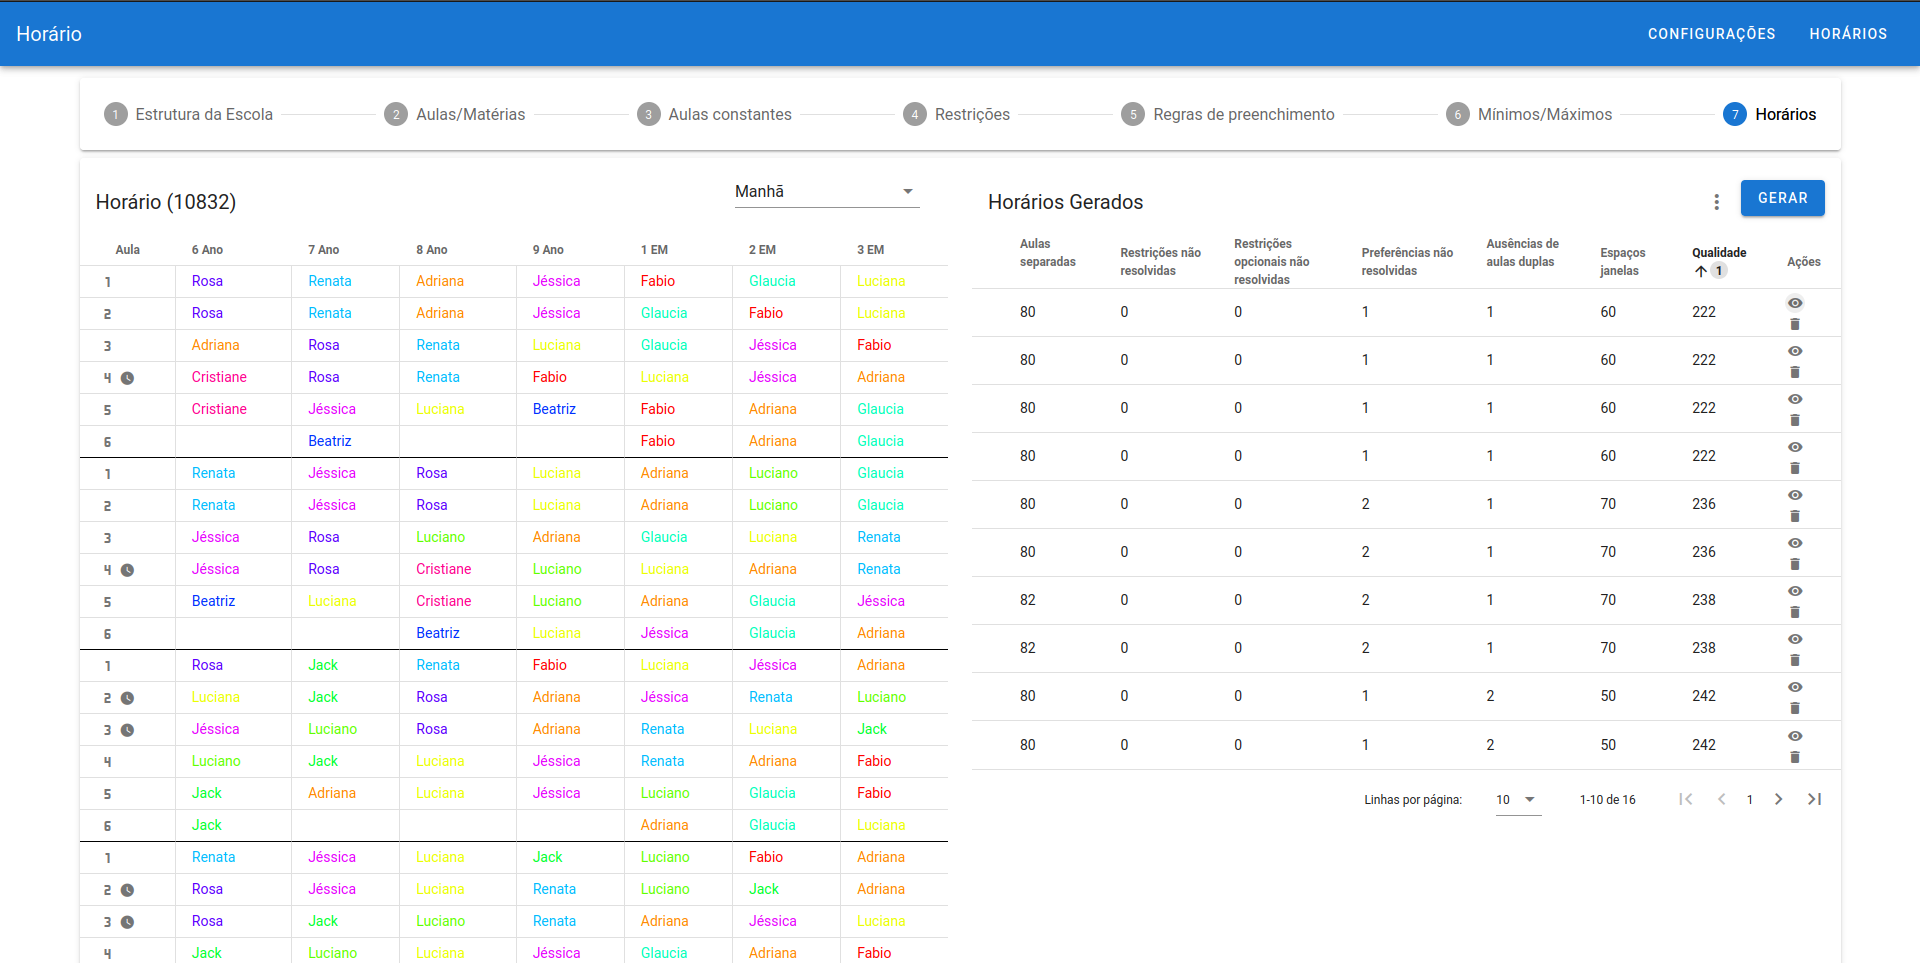
\includegraphics[width=0.8\textwidth]{./dados/figuras/tela_horarios}
	\fonte{Autor}
	\label{fig:tela-horarios}
\end{figure}
\newpage

\subsection{Servidor}
O servidor será responsável por receber as requisições da interface, persistir as configurações no banco de dados e realizar a comunicação com o otimizador, a fim de produzir e armazenar as grades horárias.

Para o desenvolvimento deste componente, optou-se pelo \textit{framework Express.js}, a ser executado na plataforma \textit{Node.js}, devido à simplicidade de implementação que estas tecnologias proporcionam. Em relação ao banco de dados, será utilizado o sistema de gerenciamento de banco de dados \textit{PostgresSQL}, devido à sua robustez.

Conforme as premissas do problema sendo tratado, a modelagem do banco de dados é centrada na entidade ``Configuração'', que agrupa as configurações de determinada instituição de ensino para a geração de suas grades horárias. Cada uma dessas entidades tem turnos, salas, professores, e as configurações de quantas aulas cada professor deve ministrar em cada sala, e as respectivas restrições.

A modelagem comentada está representada na \autoref{fig:diagrama-er}:

\begin{figure}[!htb]
	\centering
	\caption{Modelo Entidade-Relacionamento}
	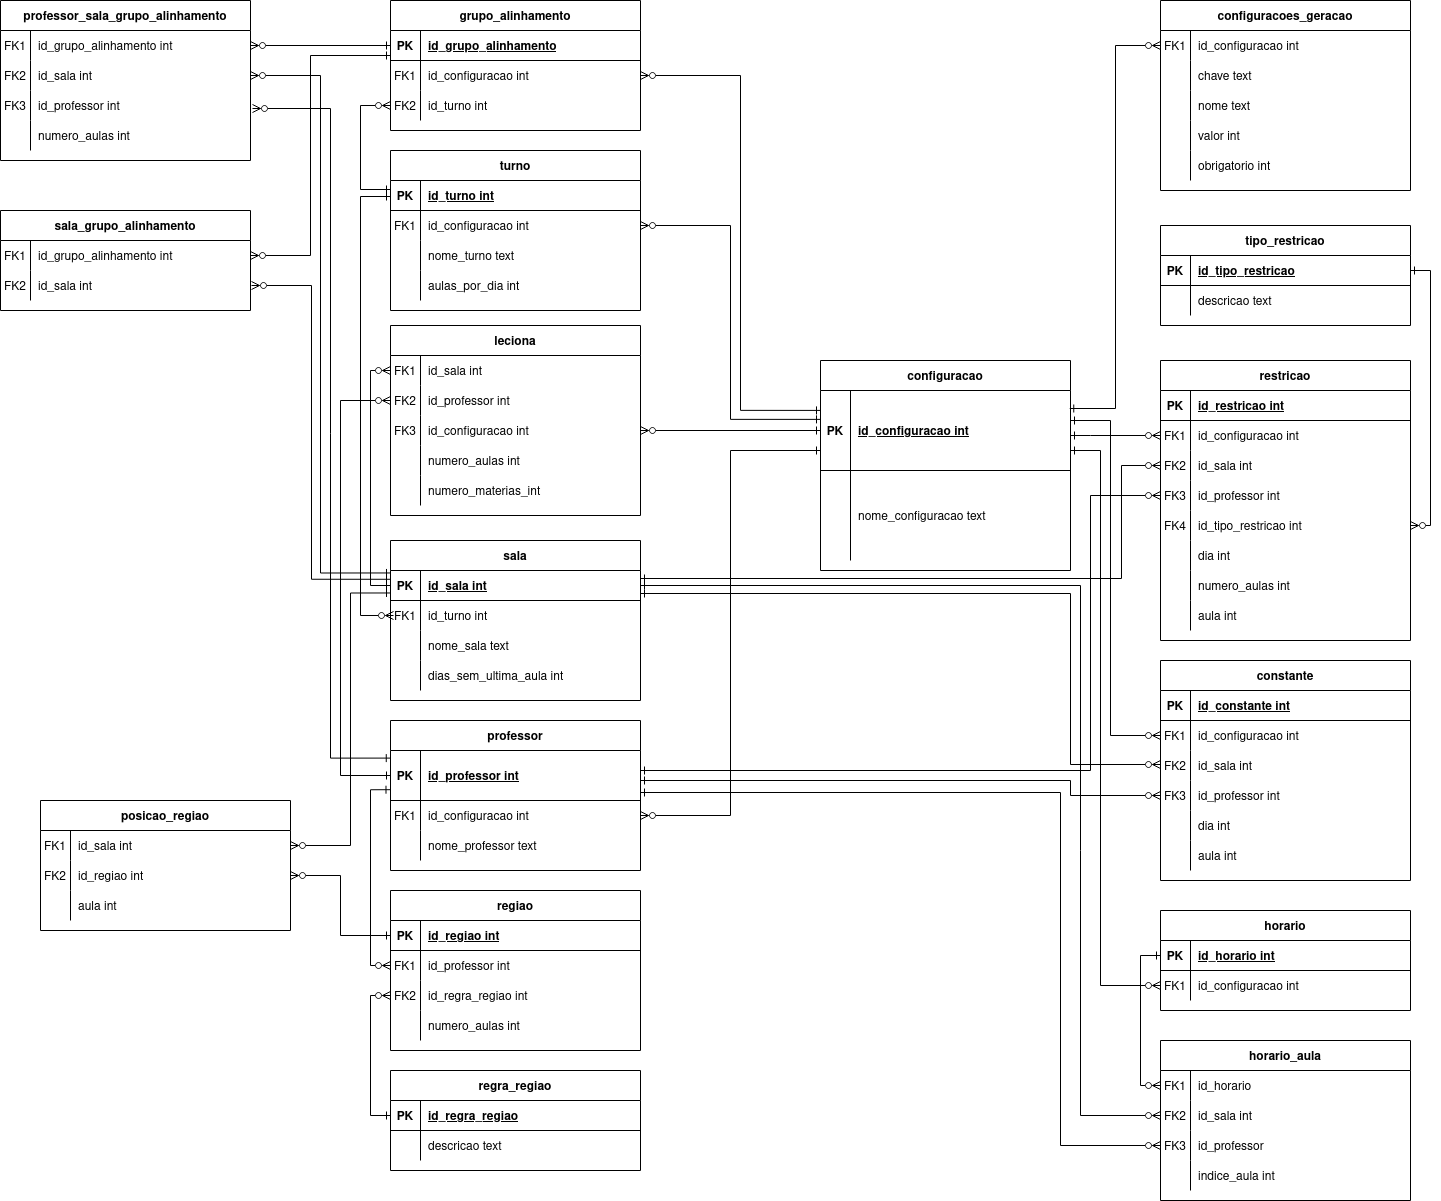
\includegraphics[width=1\textwidth]{./dados/figuras/diagrama_er}
	\fonte{Autor}
	\label{fig:diagrama-er}
\end{figure}
\newpage

Dentre as entidades mostradas no modelo entidade-relacionamento, vale ressaltar a importância da entidade ``Grupo Alinhamento''. Esta será utilizada para configurar aulas que devam acontecer simultaneamente, a fim de resolver o desafio dos itinerários formativos do Novo Ensino Médio, conforme exposto na seção \ref{sec:novo_ensino_medio}.

Para validar a modelagem do banco de dados, realizaram-se inserções de informações de exemplo nas diferentes tabelas. A \autoref{fig:sql-validacao} mostra algumas dessas inserções e os vínculos instituídos pelos identificadores escolhidos.

\begin{figure}[!htb]
	\centering
	\caption{Consultas de validação da modelagem}
	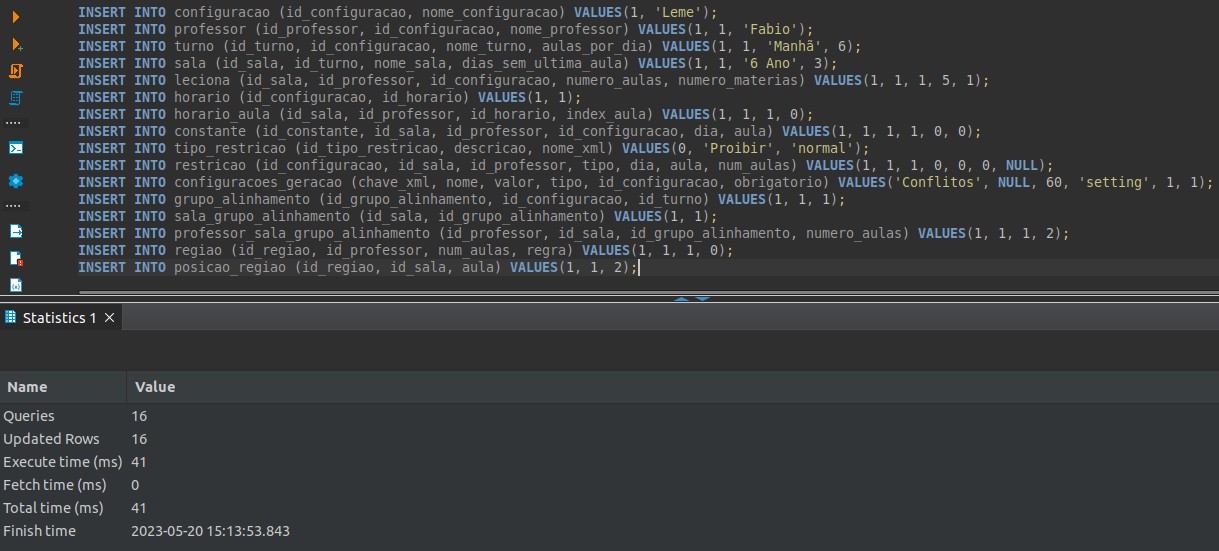
\includegraphics[width=1\textwidth]{./dados/figuras/sql_validacao}
	\fonte{Autor}
	\label{fig:sql-validacao}
\end{figure}
\newpage

Validou-se também o armazenamento das grades horárias no banco de dados. A \autoref{fig:sql-grade} traz um exemplo de consulta de uma grade horária com sete salas:

\begin{figure}[!htb]
	\centering
	\caption{Consulta SQL de grade horária com sete salas}
	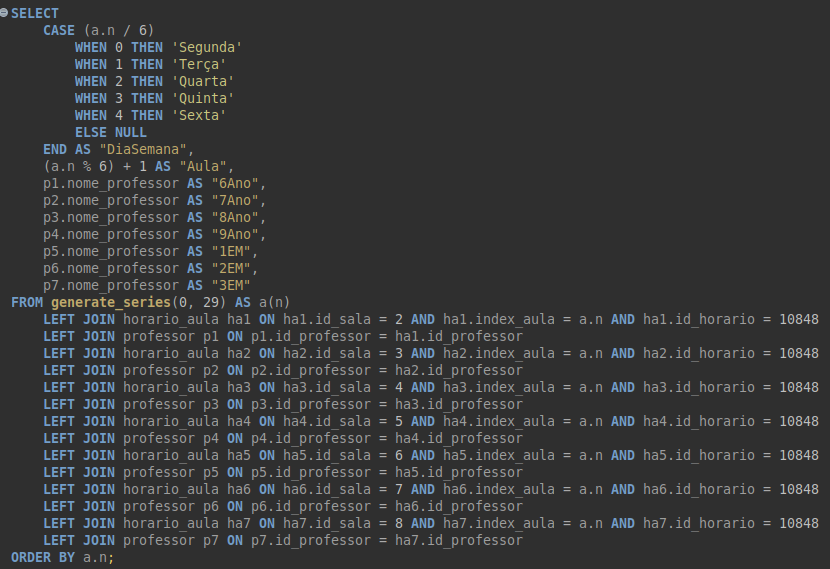
\includegraphics[width=0.7\textwidth]{./dados/figuras/sql_grade}
	\fonte{Autor}
	\label{fig:sql-grade}
\end{figure}

A consulta anterior traz como resultado a tabela visível na \autoref{fig:consulta-grade}, com linhas e colunas correpondentes a horários de aulas e salas respectivamente.

\begin{figure}[!htb]
	\centering
	\caption{Resultado da consulta de uma grade no banco de dados}
	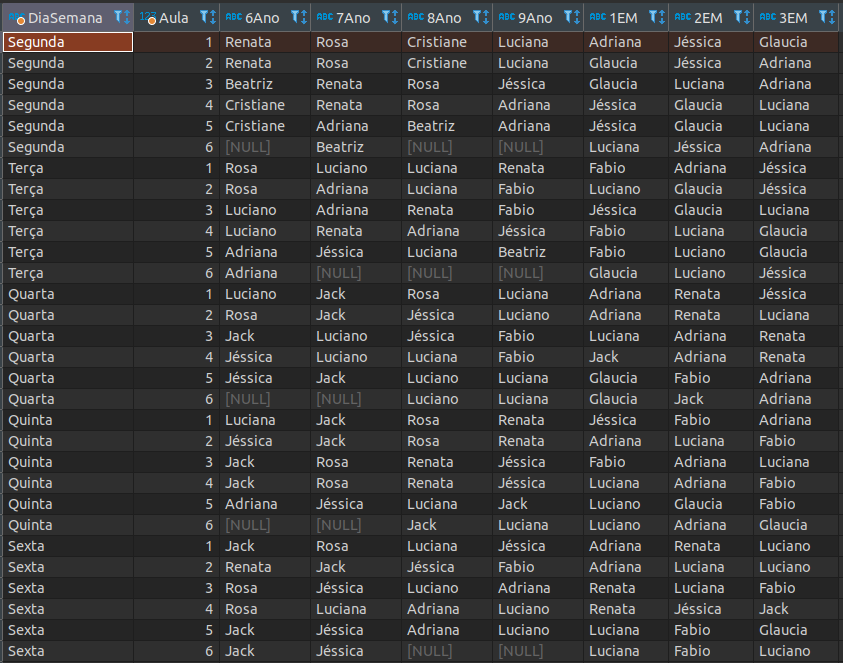
\includegraphics[width=0.7\textwidth]{./dados/figuras/ConsultaGrade}
	\fonte{Autor}
	\label{fig:consulta-grade}
\end{figure}

\newpage
\subsection{Otimizador}
O otimizador será responsável por receber as restrições formatadas pelo servidor, e gerar grades horárias adequadas com base nestas. Após a geração, os resultados devem ser enviados para o servidor para que sejam armazenados no banco de dados.

Este componente do sistema implementará um algoritmo de otimização aplicando a meta-heurística de \textit{Simulated Annealing}, a fim de gerar as soluções para o problema de otimização da grade horária conforme as configurações realizadas pelo usuário.

\section{MÉTODO}
\label{sec:metodo}
Para a processo de software da aplicação, optou-se pelo processo de desenvolvimento incremental. Este processo consiste na divisão da implementação do projeto em incrementos, os quais são executados linearmente, porém de forma escalonada.\cite{pressman2016}

Este processo de software foi escolhido por possibilitar o planejamento de execução do projeto em etapas lógicas, que podem ser sobrepor através de escalonamento, de acordo com as necessidade encontradas. Conforme os requisitos levantados na seção anterior, dividiram-se as tarefas de desenvolvimento nos incrementos pertinentes:
\begin{itemize}
	\item \textbf{Incremento 1}: Desenvolvimento inicial do otimizador, aplicando Simulated Annealing apenas para a resolução de conflitos;
	\item \textbf{Incremento 2}: Implementação de restrições no otimizador;
	\item \textbf{Incremento 3}: Criação do servidor e banco de dados;
	\item \textbf{Incremento 4}: Desenvolvimento da interface \textit{web};
	\item \textbf{Incremento 5}: Adição do sistema de usuários;
	\item \textbf{Incremento 6}: Adaptação da modelagem para incluir matérias aos horários alocados pelo otimizador;
	\item \textbf{Incremento 7}: Implementação de validações das configurações de grade inseridas pelo usuário;
	\item \textbf{Incremento 8}: Desenvolvimento de sistema de exportação de grades horárias.
\end{itemize}

Conforme evidenciado na seção \ref{sec:analise_e_desenvolvimento}, os quatro primeiros incrementos já foram executados, a fim de prototipar o sistema e verificar a viabilidade a solução planejada.

Quanto à validação do software desenvolvido, esta será realizada através de experimentos controlados, simulando requisitos das grades horárias. Após esta etapa, serão conduzidas validações no contexto de instituições de ensino reais que sejam pertinentes ao trabalho.
